%% ----------------------------------------------------------------------------
%%  §11.1  Serie numeriche
%% ----------------------------------------------------------------------------
\section{Serie numeriche}
\label{sec:serie-numeriche}

Sia $a_{n}$ una successione di numeri reali. Vogliamo dare un significato alla «somma di
tutti i suoi termini»
\begin{equation}\label{eq:serie-formale}
  a_{1}+a_{2}+a_{3}+\dots+a_{n}+\cdots .
\end{equation}
L'idea è di sommare i termini uno alla volta, osservando come si comportano le somme
così ottenute.

\begin{definizione}[Serie, somme parziali, carattere]\label{def:serie}
\index{serie}\index{serie!somma parziale}\index{serie!carattere}
Data una successione $a_{n}$, la \emph{somma parziale} (o \emph{ridotta}) $n$-esima è
\begin{equation}\label{eq:somma-parziale}
  s_{n}=a_{1}+a_{2}+\dots+a_{n}=\sum_{k=1}^{n}a_{k} .
\end{equation}
La successione $s_{n}$ si chiama \emph{serie di termine generale $a_{n}$} e si indica con
$\sum_{k=1}^{\infty}a_{k}$. La serie si dice
\begin{itemize}
  \item \emph{convergente}, se $s_{n}$ ha limite finito $s$; il numero $s$ si chiama
  \emph{somma} della serie e si scrive
  \begin{equation}\label{eq:somma-serie}
    \sum_{k=1}^{\infty}a_{k}=\lim_{n\to+\infty}s_{n}=\lim_{n\to+\infty}\sum_{k=1}^{n}a_{k}=s ;
  \end{equation}
  \item \emph{divergente} (positivamente o negativamente), se $s_{n}\to+\infty$ oppure
  $s_{n}\to-\infty$, e si scrive $\sum_{k=1}^{\infty}a_{k}=+\infty$ oppure $-\infty$;
  \item \emph{indeterminata}, se $s_{n}$ non ha limite.
\end{itemize}
Una serie convergente o divergente si dice \emph{regolare}. Il \emph{carattere} di una
serie è la proprietà di essere convergente, divergente oppure indeterminata.
\end{definizione}

Il simbolo $\sum_{k=1}^{\infty}a_{k}$ indica dunque due cose diverse: la serie, cioè la
successione delle somme parziali, e, quando esiste, la sua somma. Il contesto chiarisce
sempre di quale si tratti. Spesso conviene far partire l'indice da $0$ o da un altro
intero $k_{0}$: si scrive allora $\sum_{k=0}^{\infty}a_{k}$ o $\sum_{k=k_{0}}^{\infty}a_{k}$, con
le ovvie modifiche nella definizione delle somme parziali. Si noti infine che una serie
non è altro che una successione (quella delle somme parziali); viceversa ogni successione
$s_{n}$ è la successione delle somme parziali della serie di termine generale $a_{1}=s_{1}$,
$a_{k}=s_{k}-s_{k-1}$ per $k\ge2$. Lo studio delle serie è quindi un capitolo dello studio
delle successioni, ma con un punto di vista diverso: i dati sono i \emph{termini} $a_{k}$, e
la successione $s_{n}$ va dedotta da essi.

\begin{esempio}[La serie di Mengoli]\label{es:mengoli}\index{serie!di Mengoli}
Consideriamo la serie
\begin{equation}\label{eq:mengoli}
  \sum_{k=1}^{\infty}\frac1{k(k+1)}=\frac1{1\cdot2}+\frac1{2\cdot3}+\frac1{3\cdot4}+\dots
\end{equation}
Per la \cref{prop:telescopica}, dimostrata per induzione nel \cref{cap:numeri},
$s_{n}=\frac n{n+1}$, che tende a $1$: la serie è convergente e la sua somma vale $1$. Il
risultato si capisce meglio osservando che $\frac1{k(k+1)}=\frac1k-\frac1{k+1}$: nella somma
parziale
\[
  s_{n}=\Bigl(1-\frac12\Bigr)+\Bigl(\frac12-\frac13\Bigr)+\dots+\Bigl(\frac1n-\frac1{n+1}\Bigr)=1-\frac1{n+1}
\]
tutti i termini intermedi si elidono a due a due.
\end{esempio}

\begin{esempio}\label{es:serie-indeterminata}
La serie $\sum_{k=1}^{\infty}(-1)^{k}=-1+1-1+1-\cdots$ ha somme parziali $s_{1}=-1$, $s_{2}=0$,
$s_{3}=-1$, $s_{4}=0$, \dots, cioè $s_{n}=-1$ per $n$ dispari e $s_{n}=0$ per $n$ pari. La
successione $s_{n}$ non ha limite (\cref{cor:estratte-limiti-diversi}): la serie è
indeterminata.
\end{esempio}

Il fenomeno della serie di Mengoli, in cui le somme parziali si «accorciano» come un
cannocchiale, si generalizza.

\begin{proposizione}[Serie telescopiche]\label{prop:serie-telescopica}
\index{serie!telescopica}
Sia $a_{k}=b_{k}-b_{k+1}$ per ogni $k\ge1$, dove $b_{k}$ è una successione di numeri reali.
Allora $s_{n}=b_{1}-b_{n+1}$, e la serie $\sum_{k=1}^{\infty}a_{k}$ ha lo stesso carattere della
successione $b_{n}$: converge se e solo se $b_{n}$ ha limite finito $b$, e in tal caso
\begin{equation}\label{eq:serie-telescopica}
  \sum_{k=1}^{\infty}(b_{k}-b_{k+1})=b_{1}-\lim_{n\to+\infty}b_{n}=b_{1}-b ;
\end{equation}
diverge a $+\infty$ (a $-\infty$) se e solo se $b_{n}\to-\infty$ (rispettivamente $+\infty$);
è indeterminata se e solo se $b_{n}$ non ha limite.
\end{proposizione}

\begin{schema}
\Ipotesi{$a_{k}=b_{k}-b_{k+1}$ per ogni $k\ge1$.}
\Tesi{$s_{n}=b_{1}-b_{n+1}$; \ il carattere della serie è quello di $b_{n}$, e
$\sum_{k=1}^{\infty}a_{k}=b_{1}-\lim b_{n}$ quando il limite esiste.}
\end{schema}

\begin{strategia}
Basta calcolare la somma parziale: i termini $-b_{k+1}$ e $+b_{k+1}$ di due addendi
consecutivi si elidono, e restano solo il primo e l'ultimo. Poi si passa al limite.
\end{strategia}

\begin{dimostrazione}
Dimostriamo per induzione che $s_{n}=b_{1}-b_{n+1}$. Per $n=1$, $s_{1}=a_{1}=b_{1}-b_{2}$. Se
$s_{n}=b_{1}-b_{n+1}$, allora $s_{n+1}=s_{n}+a_{n+1}=b_{1}-b_{n+1}+b_{n+1}-b_{n+2}=b_{1}-b_{n+2}$. Dunque
$s_{n}=b_{1}-b_{n+1}$ per ogni $n$. Poiché $b_{1}$ è una costante, per i teoremi sulle
operazioni con i limiti (\cref{teo:operazioni-limiti,teo:operazioni-infinite}) la
successione $s_{n}$ ha limite se e solo se lo ha $b_{n+1}$, cioè $b_{n}$, e in tal caso
$\lim s_{n}=b_{1}-\lim b_{n}$, con la convenzione $b_{1}-(\pm\infty)=\mp\infty$.
\end{dimostrazione}

La serie di Mengoli corrisponde a $b_{k}=\frac1k\to0$, e la sua somma è $b_{1}=1$. La
proposizione permette di decidere il carattere di molte altre serie.

\begin{esempio}\label{es:serie-radici}
Il termine generale della serie
\begin{equation}\label{eq:serie-radici}
  \sum_{k=1}^{\infty}\frac1{\sqrt{k+1}+\sqrt k}
\end{equation}
tende a zero. Razionalizzando,
$\frac1{\sqrt{k+1}+\sqrt k}=\frac{\sqrt{k+1}-\sqrt k}{(k+1)-k}=\sqrt{k+1}-\sqrt k$, cioè $a_{k}=b_{k}-b_{k+1}$ con
$b_{k}=-\sqrt k$. Per la \cref{prop:serie-telescopica}, $s_{n}=\sqrt{n+1}-1\to+\infty$: la serie
\emph{diverge}, pur avendo il termine generale infinitesimo.
\end{esempio}

Nella serie indeterminata dell'\cref{es:serie-indeterminata} il termine generale $(-1)^{k}$
non tende a zero. Non è un caso: se i termini non diventano piccoli, le somme parziali
non possono stabilizzarsi.

\begin{teorema}[Condizione necessaria per la convergenza]\label{teo:condizione-necessaria}
\index{serie!condizione necessaria per la convergenza}
Se la serie $\sum_{k=1}^{\infty}a_{k}$ è convergente, allora $\lim_{n\to+\infty}a_{n}=0$.
\end{teorema}

\begin{schema}
\Ipotesi{$s_{n}=\sum_{k=1}^{n}a_{k}\to s\in\R$.}
\Tesi{$a_{n}\to0$.}
\end{schema}

\begin{strategia}
Il termine $a_{n+1}$ è la differenza di due somme parziali consecutive,
$a_{n+1}=s_{n+1}-s_{n}$. Se le somme parziali convergono a $s$, la loro differenza tende a
$s-s=0$.
\end{strategia}

\begin{dimostrazione}
Sia $s$ la somma della serie. Per ogni $n\in\N$ si ha $s_{n+1}=s_{n}+a_{n+1}$. Le successioni
$s_{n}$ e $s_{n+1}$ convergono entrambe a $s$ (la seconda è la prima con gli indici
traslati di uno), e quindi, per il teorema sul limite della differenza
(\cref{teo:operazioni-limiti}),
\[
  \lim_{n\to+\infty}a_{n+1}=\lim_{n\to+\infty}s_{n+1}-\lim_{n\to+\infty}s_{n}=s-s=0 .
\]
Dunque anche $a_{n}\to0$.
\end{dimostrazione}

\begin{attenzione}
La condizione $a_{n}\to0$ è \emph{necessaria} ma \emph{non sufficiente} per la convergenza:
la serie \eqref{eq:serie-radici} ha il termine generale infinitesimo ed è divergente.
Il teorema si usa quindi soltanto «in negativo»: se $a_{n}$ non tende a zero, la serie
certamente non converge. Se invece $a_{n}\to0$, non si può concludere nulla, e occorre
un'analisi più fine. È uno degli errori più frequenti all'esame.
\end{attenzione}

\begin{figure}[htb]
\centering
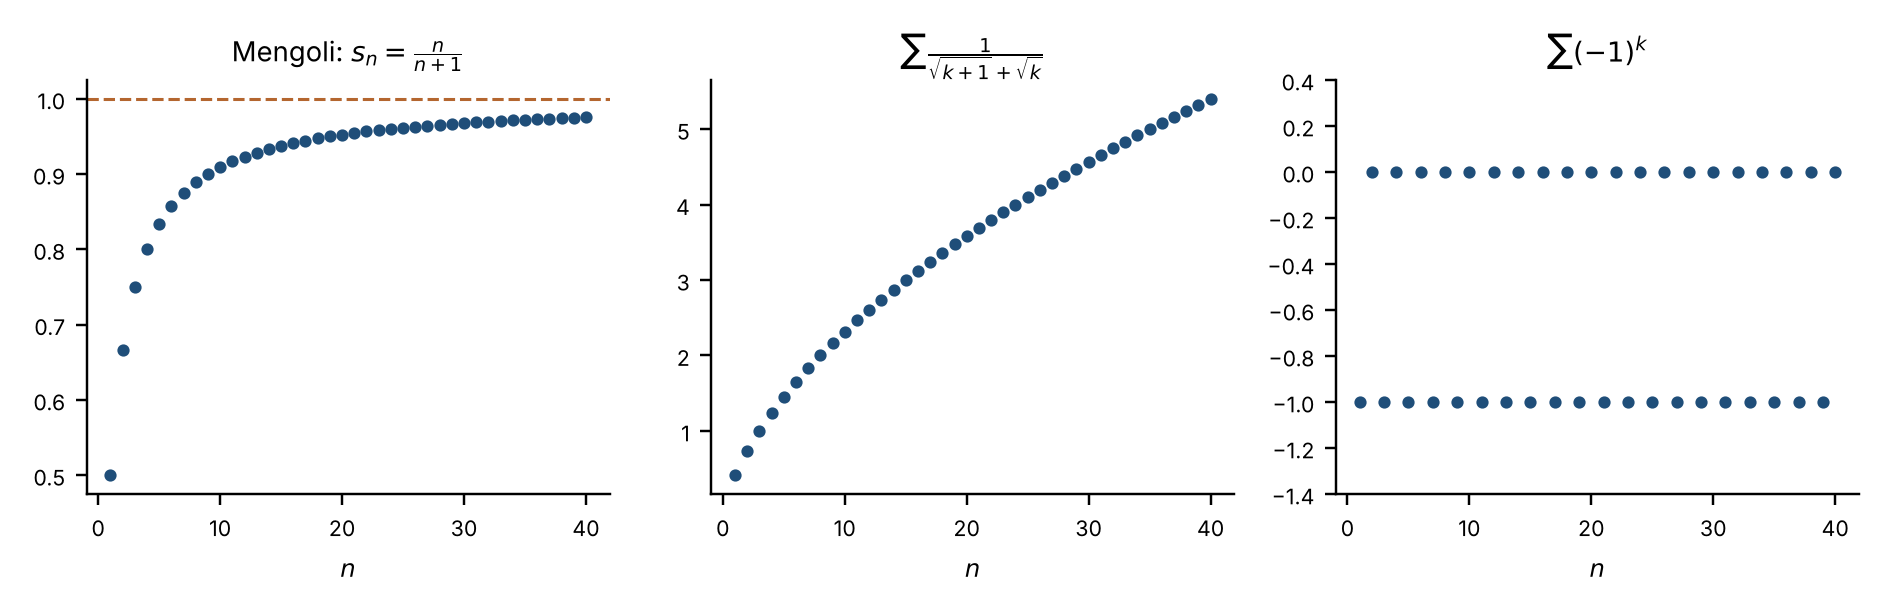
\includegraphics[width=\textwidth]{figure/somme_parziali.png}
\caption{Le somme parziali di tre serie. A sinistra la serie di Mengoli: $s_{n}=\frac n{n+1}$
converge a $1$. Al centro la serie \eqref{eq:serie-radici}: $s_{n}=\sqrt{n+1}-1$ diverge, pur
con termini che tendono a zero. A destra la serie $\sum(-1)^{k}$: le somme parziali
oscillano tra $-1$ e $0$ (\texttt{python/fig\_somme\_parziali.py}).}
\label{fig:somme-parziali}
\end{figure}

\begin{python}[Somme parziali di alcune serie]
import math

def somme_parziali(a, N):
    """Restituisce la lista s_1, ..., s_N delle somme parziali."""
    s, out = 0.0, []
    for k in range(1, N + 1):
        s += a(k)
        out.append(s)
    return out

serie = {
    "Mengoli": lambda k: 1 / (k * (k + 1)),
    "radici":  lambda k: 1 / (math.sqrt(k + 1) + math.sqrt(k)),
    "(-1)^k":  lambda k: (-1)**k,
}
for nome, a in serie.items():
    s = somme_parziali(a, 10000)
    print(f"{nome:8s}: s_10 = {s[9]:9.5f}  s_100 = {s[99]:9.5f}"
          f"  s_10000 = {s[-1]:9.5f}")
\end{python}
\begin{risultato}
Mengoli : s_10 =   0.90909  s_100 =   0.99010  s_10000 =   0.99990
radici  : s_10 =   2.31662  s_100 =   9.04988  s_10000 =  99.00500
(-1)^k  : s_10 =   0.00000  s_100 =   0.00000  s_10000 =   0.00000
\end{risultato}

\needspace{8\baselineskip}
\begin{notastorica}[Da Zenone a Mengoli]
I paradossi di Zenone di Elea (V secolo a.C.), noti attraverso la \emph{Fisica} di
Aristotele, mostrano quanto antica sia la difficoltà di pensare una somma di infiniti
termini. Archimede, nella \emph{Quadratura della parabola}, calcolò di fatto la somma
della serie geometrica $1+\frac14+\frac1{16}+\cdots=\frac43$, evitando però accuratamente
l'infinito con un ragionamento per assurdo (lo abbiamo ripercorso nel
\S\ref{subsec:archimede-parabola}). Non risulta invece che nell'antichità i
paradossi di Zenone siano stati discussi con la serie geometrica: la lettura che ne
daremo nel \S\ref{sec:serie-geometrica} è moderna. Il primo studio sistematico di serie
numeriche si deve al bolognese Pietro Mengoli, allievo di Bonaventura Cavalieri, che nelle
\emph{Novae quadraturae arithmeticae} (1650) sommò la serie che porta il suo nome e altre
serie telescopiche, dimostrò la divergenza della serie armonica e pose il problema di
calcolare $\sum\frac1{k^{2}}$, che sarebbe stato risolto da Eulero quasi un secolo dopo.
\end{notastorica}
